\chapter{Experimentos}

\section{Análise exploratória}

\subsection{Distribuição das classes}

Antes de mais nada, analisaremos a composição do nosso conjunto de dados e como se dá
a distribuição de classes. Na figura \ref{fig:classes} temos um histograma das classes associadas
a cada tuíte.

\begin{table}[H]
	\begin{center}
		\begin{tabular}{| l | l |}
			\hline
			Classe & Total \\
			\hline
			Positivo & 115 \\
			\hline 
			Negativo & 1248 \\ 
			\hline
			Neutro & 1223 \\ 
			\hline
		\end{tabular}
	\end{center}
	\caption*{Quantidade de tuítes pertencentes a cada classe}
	\label{tab:distribution}
\end{table}

\begin{center}
	\begin{figure}[H]
		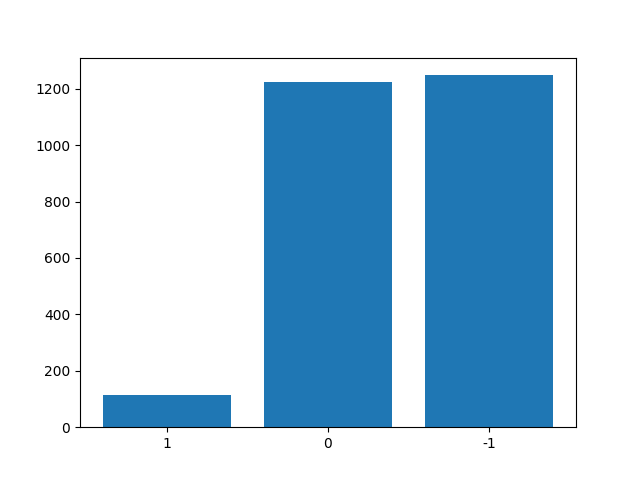
\includegraphics[scale=0.8]{fig_classes}
		\caption{Histograma da frequência de tuítes}
		\label{fig:classes}
	\end{figure}
\end{center}

Como podemos observar a partir da figura \ref{fig:classes} e tabela \ref{tab:distribution}, temos
que enquanto as classes negativa e neutra possuem distribuição próxima (48,26\% e 47,29\% 
respectivamente) a classe positiva corresponde a apenas 4,45\% de todos os tuítes. Mais a frente
veremos que esse desbalanceamento entre as classes irá acarretar em um desempenho ruim por parte
dos algoritmos de classificação, sejam os desenvolvidos para este trabalho quanto os da biblioteca
\texttt{scipy}.

\subsection{Características dos tuítes de cada classe}

A fim de entender como os classificadores realizariam o treinamento, analisou-se o conjunto de
dados a procura de padrões de características para cada classe.

Para os tuítes avaliados como neutro, notou-se o padrão que são tuítes derivados de portais de 
notícias ou são indagações, porém sem nenhuma crítica feita nelas.
A tabela abaixo mostra como exemplo alguns tuítes avaliados como neutro.

\begin{center}
	\begin{tabular}{| l | p{0.8\linewidth} |}
		\hline
		usuário & tuíte \\
		\hline
		Tica_Fernandes & Cidades têm protestos contra reforma da Previdência e terceirização http://g1.globo.com/politica/noticia/cidades-tem-protestos-contra-reforma-da-previdencia-e-terceirizacao.ghtml \\
		\hline
		andrcolett & Transposição do rio São Francisco, reforma do ensino médio/ da previdência , operação carne fraca, terceirização ... Enem vai bombar esse ano \\
		\hline
		VictoorAugustoo & Via @estadao : Manifestantes protestam em capitais do País contra reforma da Previdência e terceirização - http:/ln.is/estadao.com.brb29w1 \\
		\hline
		EdmilsonPequeno & O meu deputado @luizcoutopt votou contra a terceirização e é contra a reforma da previdência \\
		\hline
	\end{tabular}
\end{center}

Já para os tuítes negativos, nota-se a presença de palavrões e xingamentos 
junto de algumas \textit{hashtags} de cunho negativo como por exemplo \#ForaTemer,
além disso é comum a presença de tuítes onde as pessoas são convocadas para manifestações.
Outros termos comuns são escravidão e retrocesso, referindo-se diretamente às reformas da previdência e terceirização.

\begin{center}
	\begin{tabular}{| l | p{0.8\linewidth} |}
		\hline
		usuário & tuíte \\
		\hline
		MgracaGalvao & Dória é o maior Fake de todos os tempos. Se f... Palhaço \\
		\hline
		adamastaquio & Acorda POVO trabalhador. Previdencia + Terceirização + Reforma da CLT é P*** NO RABO DO POVO! \#ReformaTrabalhistaNÃO \\
		\hline
		TheMairaBastos & Reforma da previdência , desmonte da CLT, terceirização ,congelamento de gastos com a saúde e educação \#ForaTemerLadrao \#TemerGolpista \\
		\hline
		neyeverest & O PT esteve no poder por 14 anos o bandido do Lula e a burra da Dilma e o país está um caos pela instituição a roubalheira deles também !! \\
		\hline
		carinasotero & GREVE GERAL DIA 28/04 CONTRA RETROCESSOS DE TEMER • Reforma da Previdência • Reforma Trabalhista • Terceirização irrestrita \\
		\hline
	\end{tabular}
\end{center}

Assim como para os tuítes classificados como negativo, os tuítes positivos também eram 
caracterizados pela presença de \textit{hashtags}. Sejam elas declarando apoio a um candidato
(como \#Aecio2018 ou \#Lula2018) ou simplesmente manifestando alguma opinião positiva. 

\begin{center}
	\begin{tabular}{| l | p{0.8\linewidth} |}
		\hline
		usuário & tuíte \\
		\hline
		Verinha_Lu & É Aécio pelo Brasil !!! \#AécioPresidenteDoBrasil2018 \#EstamosComAécio \#DeusÉmaior e \#VitóriaVem \#FÉ \#SouAécio \\
		\hline
		Haddad_Femando & O salário mínimo aumentou 71\% durante os governos Lula e Dilma \#BrasilQueOPovoQuer \\
		\hline
		rovisacro & A favor da terceirização e tmb da reforma da previdência ! Mas óbvio, de forma justa e igualitária para todos, principalmente na previdência \\
		\hline	
	\end{tabular}
\end{center}

\section{Descrição dos experimentos}

Realizou-se duas etapas de experimentos, uma primeira etapa utilizando todas as classes onde se
observou que a baixa quantidade de elementos da classe positiva acabava por atrapalhar o desempenho
geral dos algoritmos, em especial os que utilizavam a abordagem OVA para o caso de multiclasses.
Com isso, decidiu-se descartar esses elementos e rodar uma nova sequência de experimentos 
considerando apenas as classes negativa e neutra (que para efeito dos algoritmos será a classe 
positiva) e, com isso, verificar a melhoria dos algoritmos nas métricas.

Para ambas as etapas, procurou-se não só medir o desempenho dos algoritmos, mas também encontrar
uma escolha certa de parâmetros para os mesmos que obtivesse a melhor performance (como a escolha
do Kernel no caso do SVM ou a constante de regularização usada tanto no SVM quanto na regressão
logística).

Tais testes de escolha de parâmetro, caso feitos usando apenas a divisão do conjunto de dados entre
conjunto de treino e conjunto de testes acabaria por dar uma escolha enviesada de parâmetros, uma
vez que uma escolha de parâmetros que tenha bons números em determinado conjunto de testes não
indica que ele possui uma boa generalização, isto é, apresentará uma boa precisão para novos dados.

A fim de garantir maior generalização, utiliza-se um método de validação chamado de 
validação cruzada, que se consiste de um modo de dividir o conjunto de dados e testá-lo com
um conjunto de validação. Uma primeira abordagem da validação cruzada seria dividir nosso conjunto
em três: um de treino, um de validação e outro de teste, assim testaríamos as escolhas de parâmetros
no conjunto de treino e, por fim, mediríamos a performance do melhor no conjunto de teste.

Outra abordagem seria ainda manter a divisão do conjunto de dados em conjunto de treino e teste
porém realizar esse procedimento diversas vezes alternando as porções que irão corresponder a
cada conjunto. Tal método é chamado de k-fold. No k-fold divide-se o conjunto total em k partições
e, a cada iteração, é construído um conjunto de teste usando uma das partições enquanto as k-1
serão o de treino. O procedimento de treinamento é realizado k vezes e, a escolha de parâmetros
com melhor desempenho médio será a escolhida. A figura \ref{fig:kfold} mostra o funcionamento do
método.

\begin{figure}[H]
	\begin{center}
		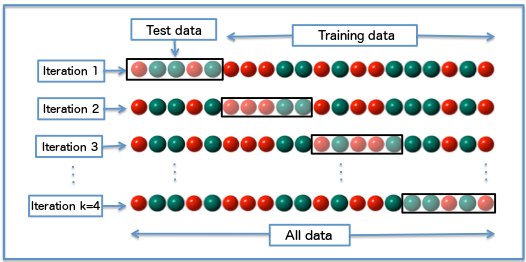
\includegraphics[scale=0.8]{K-fold_cross_validation}
	\end{center}		
	\caption{Funcionamento do método k-fold da validação cruzada \\
		fonte: \url{https://en.wikipedia.org/wiki/Cross-validation_(statistics)\#/media/File:K-fold_cross_validation_EN.jpg}}
	\label{fig:kfold}
\end{figure}

\subsection{Parâmetros avaliados}

\textbf{SVM}

Para o SVM, textou-se o desempenho do algoritmo testando diferentes kernels e com diferentes
parâmetros para cada um. Os seguintes kernels foram utilizados:

\begin{itemize}
	\item Kernel Linear: $K(x, y) = x^Ty$
	\item Kernel RBF: $K(x, y) = exp(-\gamma||x - y||^2)$
	\item Kernel Polinomial: $K(x, y) = (x^Ty + c)^d$
\end{itemize}

Em comum a todos os kernels, variou-se o parâmetro C do SVM utilizado para penalizar os valores
mal classificados. Já para o RBF, varia-se o parâmetro $\gamma$. Por último para o polinomial,
varia-se tanto o parâmetro d que determina o grau do polinômio (aqui variamos entre 3, 4 e 5) e o coeficiente.

\textbf{Regressão Logística}

Para a regressão logística, adicionamos um parâmetro extra $\lambda$ que será usado para penalizar
nosso vetor de pesos e assim, evitar \textit{overfitting}, que ocorre quando um modelo apresenta
baixo erro no conjunto de treino, porém baixa generalização. 
Importante ressaltar que $\lambda$ só é aplicado nos índices
de $1$ a $m + 1$ do vetor de pesos, com o valor do termo $w_0$ não sendo penalizado.


\section{Métricas avaliadas}

Para a realização dos experimentos, levou-se em consideração quatro métricas
para avaliar a eficiência dos classificadores.

\begin{itemize}
	\item Acurácia: taxa calculada pela quantidade de dados corretamente classificados
	sobre o total de dados. Quanto mais próximo de 1, melhor a precisão.
	\item Precisão: taxa calculada pela expressão $\frac{tp}{tp + fp}$ onde tp corresponde
	aos verdadeiro positivos, isto é, elementos corretamente classificados como da classe C
	e fp são elementos erroneamente classificados na classe C. Quanto mais próximo de 1, melhor.
	\item Revocação: taxa calculada pela expressão $\frac{tp}{tp + fn}$ onde tp corresponde
	aos verdadeiro positivos, como na precisão e fn corresponde
	aos falso negativos, isto é, os elementos incorretamente classificados como não pertencentes
	a uma classe C quando na verdade pertencem. Assim como a precisão, quanto mais próximo de
	1, melhor.
	\item Medida F: pode ser interpretado como uma média harmônica entre precisão e revocação é dado
	pela expressão: $2*\frac{precis*revocação}{precis + revocação}$. Assim como as demais medidas, quanto
	mais próximo de 1, melhor o valor.
\end{itemize}

\section{Primeiro experimento}

Nesse primeiro experimento, avaliou-se o desempenho dos classificadores desenvolvidos quanto dos
já disponíveis pela biblioteca \texttt{scikit} a fim de comparar o desempenho das implementações.
Além disso, testou-se diferentes escolhas de parâmetro para cada abordagem de vetorizar o corpus
que no caso foram vetor binário, vetor de frequência e vetor com os valores tf-idf conforme descrito
em \ref{subsec:featurization}. 
Note que neste primeiro experimento, todos os dados foram tratados \textit{in-natura}, sem nenhum método de seleção de características ou qualquer abordagem semelhante a fim de melhorar o desempenho.

\subsection{Algoritmos próprios}

Dos algoritmos desenvolvidos para este trabalho, por questão do tempo levado a cada rodada de testes
acabou dificultando a execução de múltiplas interações do algoritmo, porém testou-se o SVM 
utilizando um valor para $\gamma$ que apresentou bom desempenho na implementação do \texttt{scikit}.
E a partir dele, mediu-se acurácia, precisão, revocação e f1-score para cada classe.

Testou-se o kernel RBF com $\gamma = 10^{-4}$ e $C = 10$ utilizando
uma vetorização baseada na frequência dos termos, foi obtida uma acurácia média de 46.8\%.

\begin{table}[H]
	\centering
	\begin{tabular}{l | l | l | l | l}
		\hline
		classe  	&	precision  &  recall &  f1\-score &  support \\
		\hline
         -1   &    0.47  &    1.00   &   0.64   &    306 \\
         \hline
          0   &    0.00   &   0.00   &   0.00    &   312 \\
          \hline
          1   &    0.00   &   0.00   &   0.00    &    29 \\
		\hline
		média / total   &    0.22   &   0.47   &   0.30   &    647 \\
		\hline
	\end{tabular}
\end{table}

Pelos resultados do experimento, percebe-se que a implementação do SVM multiclasses usando a
abordagem OVA priorizou a classe negativa dando maiores valores para ela constatado pelo valor do 
revocação de -1, uma vez que quanto maior o valor maior as chances de recuperarmos um elemento
de determinada classe. Interpretamos também, por outro lado, que o classificador desconsiderou as 
demais classes, visto pelos valores das mesmas.

Cre-se que é possível implementar melhorias no método OVA para que esse desbalanceio não seja tão
drástico, ou até mesmo normalizar os valores de $y_k$ para cada classe k de modo que seja possível
garantir que estão em faixas de valores próximos, pois um dos perigos dessa abordagem é que cada
classificador gere valores de magnitudes diferentes uns dos outros e assim enviesando a comparação
entre si.

Além disso, também existe mais espaço para melhorias no resultado utilizando outras escolhas de Kernel
ou até mesmo escolha de outros valores para $\gamma$ usando o Kernel RBF.

\subsection{Implementações do \texttt{scikit}}

Abaixo, separaremos os testes baseados em como a obtenção do vetor de \textit{features} foi feita
ao invés dos algoritmos, uma vez que para todos esses realizou-se os mesmos testes. Importante 
ressaltar que só serão colocados aqui os melhores resultados de cada um, uma vez que existe uma
grande quantidade de resultados. 

Os resultados dos experimentos serão comentados apenas ao final desta subseção, após mostrar
os valores encontrados para todas as formas de vetorização.


\textbf{Frequência}

\begin{table}[H]
	\centering
	\caption{Resultados para o SVM}
	\begin{tabular}{l l l l}
		\hline
		Kernel & C & parâmetros & Acurácia média \\
		\hline
		Linear & 0,1 & & 0,666 \\
		\hline
		Linear & 1 & & 0,637 \\
		\hline
		RBF & 100 & $\gamma = 10^{-3}$ & 0,663 \\
		\hline
		RBF & 100 & $\gamma = \frac{1}{\# amostras}$ & 0,653 \\
		\hline
		Polinomial & 0,01 & $c = 10$, $d = 5$ & 0,666 \\
		\hline
		Polinomial & 100 & $c = 1$, $d = 4$ & 0,663 \\
		\hline
	\end{tabular}
\end{table}

Importante ressaltar que em casos de empate, o primeiro melhor será selecionado, no caso o melhor
foi o kernel linear com $C = 0.1$, utilizando esses valores no conjunto de testes obteve-se os 
seguintes resultados:

\begin{table}[H]
	\centering
		\begin{tabular}{l | l | l | l | l}
		\hline
		classe  	&	precisão  &  recall &  f1\-score &  support \\
		\hline		
		 -1     &  0.70  &    0.73   &   0.71   &    324 \\
		  \hline
          0     &  0.67   &   0.69   &   0.68    &   298 \\
          \hline
          1     &  1.00   &   0.04   &   0.08    &    25 \\
			\hline
		média / total     &  0.70  &    0.68  &    0.67   &    647 \\
		\hline
	\end{tabular}
\end{table}

Para a regressão logística, variou-se o valor de $\lambda$ entre $10^{-4}$ a $1$ e, além disso
variou-se a abordagem para o caso multiclasses, uma vez que o \texttt{scikit} disponibiliza
uma implementação usando o método OVA e outro usando o método multinomial (assim como implementou-se).

\begin{table}[H]
	\centering
	\caption{Resultados da regressão logística}
	\begin{tabular}{l l l}
		\hline
		Método & $\lambda$ & Acurácia média \\
		\hline
		OVA & 0.1 & 0.654 \\
		\hline
		OVA & 1 & 0.651 \\
		\hline
		Multinomial & 0.1 & 0.654 \\
		\hline
		Multinomial & 1 & 0.649 \\
		\hline
	\end{tabular}
\end{table}

Assim como para o SVM, escolheu-se o primeiro melhor que no caso é a abordagem OVA com $\lambda = 0.1$.
Deu os seguintes resultados no conjunto de testes:

\begin{table}[H]
	\centering
		\begin{tabular}{l | l | l | l | l}
		\hline
		classe  	&	precisão  &  recall &  f1\-score &  support \\
		\hline
         -1   &    0.70  &    0.68   &   0.69   &    320 \\
         \hline
          0    &   0.68   &   0.73   &   0.70   &    307 \\
          \hline
          1    &   0.50   &   0.15   &   0.23   &     20 \\
		\hline
		média / total  &     0.68  &    0.69    &  0.68   &    647 \\
		\hline
	\end{tabular}
\end{table}

\textbf{Vetor binário}

\begin{table}[H]
	\centering
	\caption{Resultados para o SVM}
	\begin{tabular}{l l l l}
		\hline
		Kernel & C & parâmetros & Acurácia média \\
		\hline
		Linear & 0,1 & & 0,658 \\
		\hline
		Linear & 1 & & 0,643 \\
		\hline
		RBF & 100 & $\gamma = 10^{-3}$ & 0,649 \\
		\hline
		RBF & 100 & $\gamma = \frac{1}{\# amostras}$ & 0,646 \\
		\hline
		Polinomial & 100 & $c = 1$, $d = 4$ & 0,656 \\
		\hline
		Polinomial & 1 & $c = 5$, $d = 4$ & 0,658 \\
		\hline
	\end{tabular}
\end{table}

Assim como para o vetor de frequências, a melhor escolha de parâmetros encontrada na validação
cruzada foi C = 0,1 e kernel linear. Executando no conjunto de testes obteve-se os seguintes
resultados:

\begin{table}[H]
	\centering
		\begin{tabular}{l | l | l | l | l}
		\hline
		classe  	&	precisão  &  recall &  f1\-score &  support \\
		\hline
         -1    &   0.66   &   0.76  &    0.71    &   310 \\
         \hline
          0     &  0.69   &   0.66   &   0.67    &   302 \\
         \hline
          1     &  1.00  &    0.06   &   0.11    &    35 \\
		\hline
		média / total    &   0.69   &   0.68   &   0.66    &   647 \\
		\hline
	\end{tabular}
\end{table}

\begin{table}[H]
	\centering
	\caption{Resultados da regressão logística}
	\begin{tabular}{l l l}
		\hline
		Método & $\lambda$ & Acurácia média \\
		\hline
		OVA & 0.1 & 0.631 \\
		\hline
		OVA & 1 & 0.634 \\
		\hline
		Multinomial & 0.1 & 0.631 \\
		\hline
		Multinomial & 1 & 0.630 \\
		\hline
	\end{tabular}
\end{table}

Tal qual com o vetor de frequências, escolheu-se a abordagem OVA e $\lambda = 1$ obtendo os seguintes
resultados no conjunto de testes:

\begin{table}[H]
	\centering
		\begin{tabular}{l | l | l | l | l}
		\hline
		classe  	&	precisão  &  recall &  f1\-score &  support \\
		\hline
		 -1    &   0.68   &   0.73  &    0.71   &    305 \\
		 \hline
          0    &   0.70   &   0.69   &   0.69   &    317 \\
          \hline
          1   &    0.33   &   0.04   &   0.07   &     25 \\
		 \hline
		média / total    &   0.67   &   0.69  &    0.68   &    647 \\
		\hline
	\end{tabular}
\end{table}

\textbf{Tf-idf}

\begin{table}[H]
	\centering
	\caption{Resultados para o SVM}
	\begin{tabular}{l l l l}
		\hline
		Kernel & C & parâmetros & Acurácia média \\
		\hline
		Linear & 1 & & 0,658 \\
		\hline
		Linear & 10 & & 0,627 \\
		\hline
		RBF & 100 & $\gamma = 10^{-3}$ & 0,651 \\
		\hline
		RBF & 1 & $\gamma = 10^{-4}$ & 0,483 \\
		\hline
		Polinomial & 1 & $c = 5$, $d = 5$ & 0,678 \\
		\hline
		Polinomial & 10 & $c = 10$, $d = 3$ & 0,677 \\
		\hline
	\end{tabular}
\end{table}

Com essa vetorização, diferente das demais, os melhores parâmetros escolhidos foram kernel polinomial
com coeficiente e grau 5. Utilizando esses valores, obteve-se o seguinte resultado no conjunto de
testes:

\begin{table}[H]
	\centering
		\begin{tabular}{l | l | l | l | l}
		\hline
		classe  	&	precisão  &  recall &  f1\-score &  support \\
		\hline
		 -1    &   0.64   &   0.79   &   0.71   &    311 \\
		 \hline
          0    &   0.69   &   0.60  &    0.64    &   301 \\
          \hline
          1   &    0.00   &   0.00   &   0.00    &    35 \\
          \hline
		média / total   &    0.63   &   0.66   &   0.64   &    647 \\
		\hline
	\end{tabular}
\end{table}

\begin{table}[H]
	\centering
	\caption{Resultados da regressão logística}
	\begin{tabular}{l l l}
		\hline
		Método & $\lambda$ & Acurácia média \\
		\hline
		OVA & 0.1 & 0.659 \\
		\hline
		OVA & 1 & 0.665 \\
		\hline
		Multinomial & 0.1 & 0.660 \\
		\hline
		Multinomial & 1 & 0.662 \\
		\hline
	\end{tabular}
\end{table}

Neste teste, assim como os demais usando a regressão logística, escolheu-se a abordagem OVA com
$\lambda = 1$ obtendo seguintes resultados no conjunto de testes:

\begin{table}[H]
	\centering
		\begin{tabular}{l | l | l | l | l}
		\hline
		classe  	&	precisão  &  recall &  f1\-score &  support \\
		\hline
		 -1    &   0.66   &   0.75   &   0.70   &    312 \\
		 \hline
          0    &   0.69   &   0.66   &   0.68   &    310 \\
          \hline
          1    &   0.00   &   0.00   &   0.00    &    25 \\
		\hline
		média / total   &    0.65   &   0.68   &   0.66   &    647 \\
		\hline
	\end{tabular}
\end{table}

Observa-se que, para ambos os algoritmos tem-se que nenhum valor foi classificado como
positivo quando usou-se a vetorização através do valor tf-idf de cada termo, apesar de ainda
apresentar desempenho médio aceitável. 

Isso pode ser explicado de a vetorização usando tf-idf
leva-se em consideração a relevância das palavras na sentença como um todo e, possivelmente
algumas palavras associadas a documentos positivos estão também associadas
a documentos neutros portanto não possuem um valor tf-idf alto, aliado ao fato de o vocabulário
ser montado levando em conta apenas as 5000 palavras com melhores pontuações ou presença, portanto
algumas palavras explicitamente associadas a documentos positivos não compuseram o vetor de
\textit{features}.

Por outro lado se olharmos os desempenhos utilizando frequências simples ou um vetor binário
obtemos resultados semelhantes para ambos os algoritmos, todavia ainda existe um melhor desempenho
com a vetorização por frequências tal como o SVM apresenta melhores resultados em relação à regressão
logística, mesmo que com pouca diferença.

Comum a todos os experimentos foram resultados ruins associados à classe positiva. No caso do SVM
obteve-se alta precisão em alguns casos, porém as taxas de revocação e f1-score foram baixas. Valores
baixos para revocação e f1-score podem ser interpretados como um sinal de que os classificadores
são ruins para detectar opiniões positivas. A exemplo do melhor classificador, tem-se uma taxa
de revocação de 0,08 que indica que 92\% das amostras positivas não são detectadas pelo algoritmo.

Motivado pelo baixo desempenho visto na classe positiva em todos os experimentos aliado à baixa
quantidade de tuítes nessa classe, rodou-se mais experimentos, porém dessa vez usando apenas as
outras classes.